\chapter{A Medical Case Study}\label{c:medical-study}

In this thesis we primary focus to analyze medical data by using some of the aforementioned techniques from section \ref{c:preliminaries}.
More specifically we have developed a complete system built around secure medical data analytics that could be beneficial to patients, doctors and researchers.

The system can provide insights about some medical datasets that are imported into the system to anyone who wants to query them, without compromising individual patient's privacy.
These analytics which include data aggregation / statistics and classification are implemented through privacy preserving algorithms under the secure multi-party computation scenario.

The system provides end to end work flow starting from the query selection from a user.
Following is the secure data importing, the performing of privacy preserving data analytics algorithms upon those data and finally the visualization of the results to the end user through a friendly user interface (UI).

\section{A Doctor's view}
We consider the use case of a doctor working in a hospital that wants to examine the data stored in that hospital's datasets.
She could possibly want to evaluate a treatment's outcome.
To achieve this the doctor should monitoring some particular datasets in order to have an overall view of the patients' condition over time.
This could allow a comparison between previously treated patients and enable data\hyp driven cues for the treatment.
For example a drug's effect could be evaluated that way.

The doctor could also compare aggregate results from datasets between different hospitals.
That way she could get an insight of how each patients' condition varies between different hospitals, which could indicate the different effect that different treatments have on patients and identify patterns
and differences in these treatments.

Continuous monitoring of patient data is useful for any hospital.
Provided with usable and informative tools a doctor could potentially make better diagnoses and take the appropriate action for each case.

\section{An Individual's view}
An individual could also benefit from the insights provided by our system.
We consider the case in which an individual with certain condition queries the available datasets looking for the same condition.
The individual could locate the hospitals in which patients with the same condition are treated.
Also, he could identify which hospitals in his area have the best outcome for patients with conditions similar to his.

Another way an individual could be benefited from the privacy preserving medical data analytics is the use of a classification mechanism using a model trained over patient data.
This way one could classify himself to a condition / disease or another chosen attribute for that matter, based on his own data.

\section{A Researcher's view}
We examine the case where an academic or industry researcher queries the datasets to see if they suit their research needs.
They could discover if the datasets are providing enough utility / information and decide which ones to use for performing analysis on.

For example, studying aggregate statistical information of the datasets, one could find possible correlations of particular attributes or find patterns of treatments and conditions.

A researcher could also study the relation between certain conditions and different hospitals, which is something that could provide valuable information.


%%%%%%%%%%%%%%%%%%% This does not belong in this section. It is about architecture %%%%%%%%%%%%%%%%%%%%%%%%%%%%%%%

% In such a case, the computing nodes are not necessarily the ones that also provide the data.
% Indeed, in our study, the data providers are hospitals and the computing nodes are three different servers.
% When the medical data are transferred from the hospitals to the computing nodes, a secret sharing scheme is applied; thus it is impossible for any of the three nodes to decrypt them, and in general to infer any information, as each computing node possesses only a share of the data.
% As we examined in section \ref{s:smpc}, the only requirement of the three computing parties is not to collude.
% This should not be confused with trusted servers.
% They are only trusted not to collude.
% A reasonable way to prevent collusion, is to deploy the computing nodes in premises of organizations having conflicting interests.
%
%
% After gathering the patients' data -- in secret-shared form -- the computing nodes can evaluate any arbitrary function that is deployed with respect to the SMPC model.
% Any third party or analyst, can query the cluster of nodes and request a computation.

%%%%%%%%%%%%%%%%%%%%%%%%%%%%%%%%%%%%%%%%%%%%%%%%%%%%%%%%%%%%%%%%%%

\section{Our architecture \fixme{give a fancy name for the whole scheme.}}\label{s:architecture}
Our architecture consists of the SMPC cluster (the three computing nodes) and a proxy server, dubbed \textit{coordinator}, that handles all private computation requests, as well as \texttt{N} more servers that are hosted in the data providers' premises (in our case the hospitals).
The \textit{coordinator} listens for requests for private computation, and when such a request arises, the coordinator communicates with the data providers (all \texttt{N} hospitals) requesting them securely import their data to the computing cluster.
The data are secret shared to the three parties, thus it is impossible for any of the nodes or anyone listening in the communication channel to infer the slightest information about the patients.



The detailed procedure is depicted in figure \ref{f:overview}.
First, an analyst sends a request to the \textit{coordinator} asking for a private computation, specifying an attribute and the hospitals from which the data will originate -- let us assume an aggregation over a field \texttt{X}, for hospitals \texttt{A} and \texttt{B}.
Then, the main server request from each selected hospital (in our case \texttt{A} and \texttt{B}) to import their data for attribute \texttt{X} to the SMPC cluster.
Consecutively, using an additive secret sharing protocol, the hospitals' servers securely import their data to the three computing nodes.
The actual computation takes place after the import is complete, and finally the aggregation over attribute \texttt{X} is returned to the user through the \textit{coordinator}.




\begin{figure}[th]
  \centering
  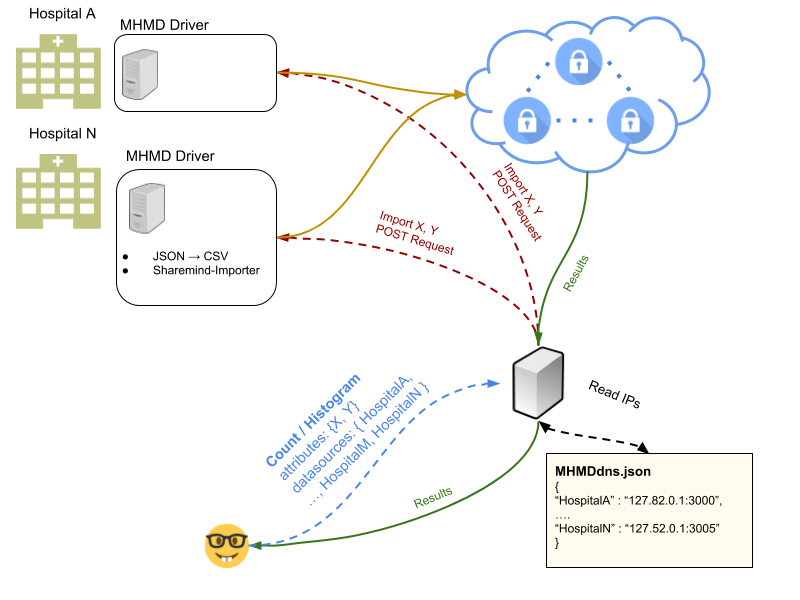
\includegraphics[width=\linewidth]{figures/overview.png}
  % \vspace{-0.2in}
  \caption{An overview of the architecture of our study \fixme{update to latest version: (not yet..)}}\label{f:overview}
\end{figure}



\section{Data Importing}\label{s:importing}
The data importing is a procedure of high importance, since the patients data are transferred outside the hospitals to third party servers.
It is easily misinterpreted that since the data are leaving the hospitals' premises, their privacy is being compromised.
However, it has been elucidated in section \ref{s:secret-sharing} that secret sharing is a form of encryption, thus no information leakage is possible while data being in transit and in use in the SMPC cluster.



\subsection{Data Importing On-the-Fly}\label{s:importing-otf}
\fixme{Why importing on the fly?}




\section{Supported Computations}\label{s:computations}
\fixme{General description of hist, id3. Details in \ref{c:pp-algorithms}
}

\fixme{what is a histogram/count and why it is usefull?}

\fixme{what is a classification tree and why it is usefull?}



